\documentclass[17pt,a4paper,landscape]{extarticle}
\usepackage[margin=2.35cm,top=0.12cm,left=1.05cm]{geometry}
\usepackage{amsmath}
\usepackage{amssymb}
\usepackage{tasks}
\usepackage{tikz}
\usepackage{xcolor}
\usepackage[sfdefault,lf]{FiraSans}
\renewcommand{\familydefault}{\sfdefault}
\setlength{\parindent}{0pt}
\pagestyle{empty}
\settasks{label=\textbf{\arabic*.}, label-width=2.2em, item-indent=2.95em, column-sep=2.1cm, after-item-skip=4.7em}
\renewcommand{\arraystretch}{1.15}
\everymath{\displaystyle}

\begin{document}
\sffamily
\boldmath

\boldmath

{\LARGE \textbf{Area of basic shapes --- Proficient}}
\begin{tasks}(3)
\task Find the area.\\[0.4em]
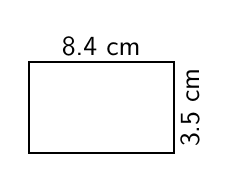
\begin{tikzpicture}[x=0.23cm,y=0.23cm,baseline=(current bounding box.center)]
  \draw[thick] (0,0) rectangle (8,5);
  \node at (4,5.9) {8.4 cm};
  \node[rotate=90] at (8.9,2.5) {3.5 cm};
\end{tikzpicture}
\task Find the area.\\[0.4em]
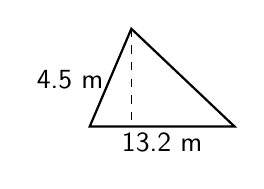
\begin{tikzpicture}[x=0.23cm,y=0.23cm,baseline=(current bounding box.center)]
  \coordinate (A) at (0,0);
  \coordinate (B) at (8,0);
  \coordinate (C) at (2.3,5.4);
  \draw[thick] (A)--(B)--(C)--cycle;
  \draw[dashed] (C)--(2.3,0);
  \node at (4,-0.9) {13.2 m};
  \node at (1.3,2.6) [left] {4.5 m};
\end{tikzpicture}
\task Find the area.\\[0.4em]
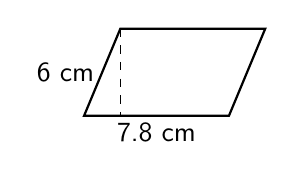
\begin{tikzpicture}[x=0.23cm,y=0.23cm,baseline=(current bounding box.center)]
  \coordinate (A) at (0,0);
  \coordinate (B) at (8,0);
  \coordinate (C) at (10,4.8);
  \coordinate (D) at (2,4.8);
  \draw[thick] (A)--(B)--(C)--(D)--cycle;
  \draw[dashed] (D)--(2,0);
  \node at (4,-0.9) {7.8 cm};
  \node at (1.1,2.4) [left] {6 cm};
\end{tikzpicture}
\task Find the area.\\[0.4em]
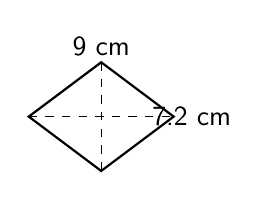
\begin{tikzpicture}[x=0.23cm,y=0.23cm,baseline=(current bounding box.center)]
  \coordinate (T) at (4,6);
  \coordinate (R) at (8,3);
  \coordinate (B) at (4,0);
  \coordinate (L) at (0,3);
  \draw[thick] (T)--(R)--(B)--(L)--cycle;
  \draw[dashed] (T)--(B);
  \draw[dashed] (L)--(R);
  \node at (4,6.9) {9 cm};
  \node at (9.0,3) {7.2 cm};
\end{tikzpicture}
\task Find the area.\\[0.4em]
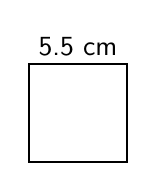
\begin{tikzpicture}[x=0.25cm,y=0.25cm,baseline=(current bounding box.center)]
  \draw[thick] (0,0) rectangle (5,5);
  \node at (2.5,5.9) {5.5 cm};
\end{tikzpicture}
\task A rectangle is 16 cm by 9 cm. Find its area.
\task A triangle has base 15 m and height 8 m. Find its area.
\task A parallelogram has base 12.5 cm and height 7 cm. Find its area.
\task A kite has diagonals 14 cm and 11 cm. Find its area.
\task The area of a rectangle is 54 cm\mbox{$^2$}. Its width is 6 cm. Find the length.
\task The area of a triangle is 36 m\mbox{$^2$}. Its base is 9 m. Find the height.
\task The area of a parallelogram is 63 cm\mbox{$^2$}. Its height is 7 cm. Find the base.
\task The area of a kite is 48 cm\mbox{$^2$}. One diagonal is 12 cm. Find the other diagonal.
\task A square has area 81 cm\mbox{$^2$}. Find the side length.
\task Which has the greater area: a rectangle \mbox{$9$} cm by \mbox{$6$} cm or a triangle with base \mbox{$14$} cm and height \mbox{$8$} cm?
\task A triangle and a parallelogram both have base 10 cm and height 6 cm. Which has the greater area, and by how much?
\task Explain why a triangle with the same base and height as a rectangle has half the area.
\end{tasks}

\end{document}
